\section{Data Sample}\label{section:star_data_sample}
Analyzed data were collected during RHIC Run 15, i.e. year 2015. During this year proton-proton centre of mass energy was equal to $\sqrt{s}=200$~GeV. Data from the RP related triggers is stored in the st\_rp data stream.  All of the studies in this work use data from only the SDT trigger condition, which was the main trigger designed for SDD studies in Run 15 and used in this analysis. Integrated luminosity delivered by the RHIC to the STAR detector in $pp$ collisions during Run 15 amounts to $185.1$~pb$^{-1}$\cite{RHIC:rhicRunLuminosity}, shown in Fig.~\ref{fig:lumiRHIC}, whereas about $34.4$M SDT events were gathered by the STAR detector, which corresponds to $16$~nb$^{-1}$ of integrated luminosity.

\begin{figure}[bh]
	\centering
	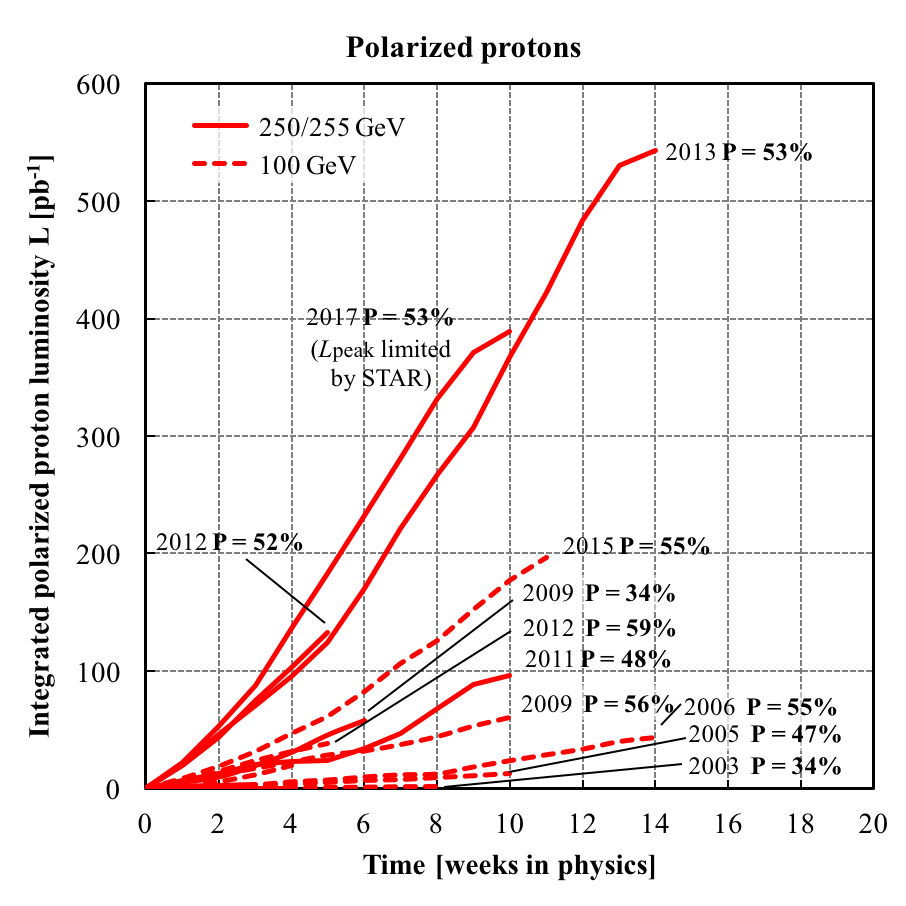
\includegraphics[width=.39\textwidth]{chapters/dataSampleSTAR/img/RhicLuminosityPP.png}
	\hfill
	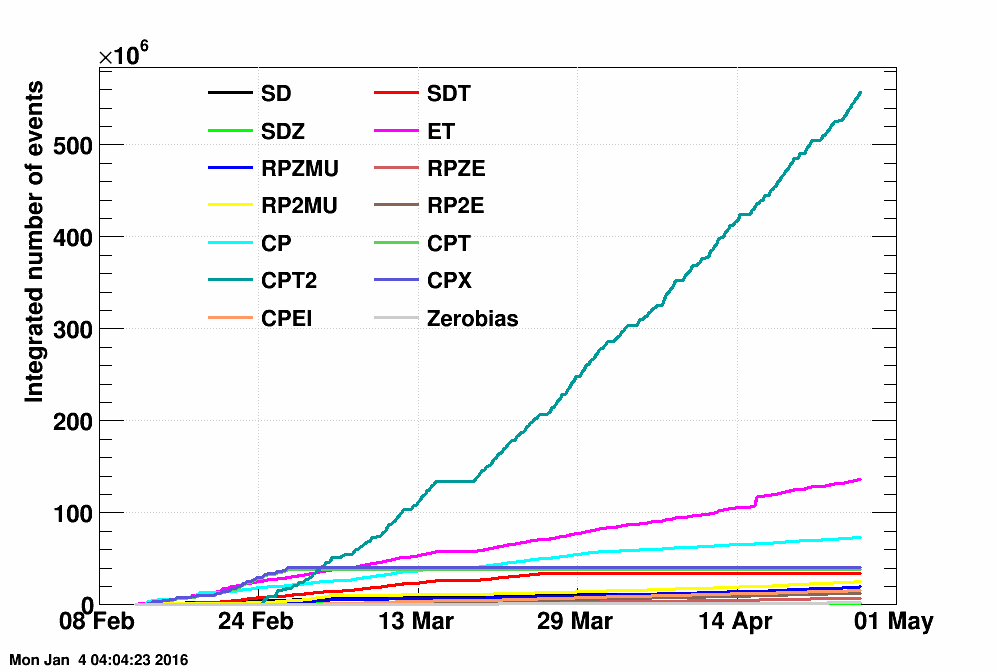
\includegraphics[width=.6\textwidth]{chapters/dataSampleSTAR/img/nEvents.png}
	\caption[Integrated luminosity delivered by the collider over the seventeen years of operation of RHIC and integrated number of events collected for each trigger in the st\_rp data stream during Run 15]{Integrated lumonosity delivered by the collider over the seventeen years of operation of RHIC (left)\cite{RHIC:rhicRunLuminosity}. Dashed lines are for $100$~GeV/c proton momentum mailnly for transverse spin physics programs, while continuous lines are for $250/255$~GeV/c proton beams aimed predominantly at the $W$-physics program. The percentage polarization reached in each run is indicated next to the curves. Integrated number of events collected for each trigger in the st\_rp data stream during Run 15 (right). About $34.4$M SDT events were gathered, which  corresponds to 16~nb$^{-1}$ of integrated luminosity.}
	\label{fig:lumiRHIC}
\end{figure}

\FloatBarrier